\documentclass{article}
\usepackage{listings}
\usepackage{mathrsfs}
\usepackage[utf8]{inputenc}
\usepackage{amssymb}
\usepackage{lipsum}
\usepackage{amsmath}
\usepackage{fancyhdr}
\usepackage{geometry}
\usepackage{scrextend}
\usepackage[english,german]{babel}
\usepackage{titling}
\setlength{\droptitle}{-3cm}
\usepackage{tikz}
\usepackage{algorithm,algpseudocode}
\usepackage[doublespacing]{setspace}
\usetikzlibrary{datavisualization}
\usetikzlibrary{datavisualization.formats.functions}
\usepackage{polynom}
\usepackage{amsmath}
\usepackage{gauss}
\usepackage{tkz-euclide}
\usetikzlibrary{datavisualization}
\usetikzlibrary{datavisualization.formats.functions}
\author{
Alexander Mattick Kennung: qi69dube\\
Kapitel 1
}
\usepackage{import}
\date{\today}
\geometry{a4paper, margin=2cm}
\usepackage{stackengine}
\parskip 1em
\newcommand\stackequal[2]{%
  \mathrel{\stackunder[2pt]{\stackon[4pt]{=}{$\scriptscriptstyle#1$}}{%
  $\scriptscriptstyle#2$}}
 }
\makeatletter
\renewcommand*\env@matrix[1][*\c@MaxMatrixCols c]{%
  \hskip -\arraycolsep
  \let\@ifnextchar\new@ifnextchar
  \array{#1}}
\makeatother
\lstset{
  language=haskell,
}
\lstnewenvironment{code}{\lstset{language=Haskell,basicstyle=\small}}{}
\usepackage{enumitem}
\setlist{nosep}
\usepackage{titlesec}

\titlespacing*{\subsection}{0pt}{2pt}{3pt}
\titlespacing*{\section}{0pt}{0pt}{5pt}
\titlespacing*{\subsubsection}{0pt}{1pt}{2pt}
\title{Vorlesung 4}


\begin{document}
	\maketitle
	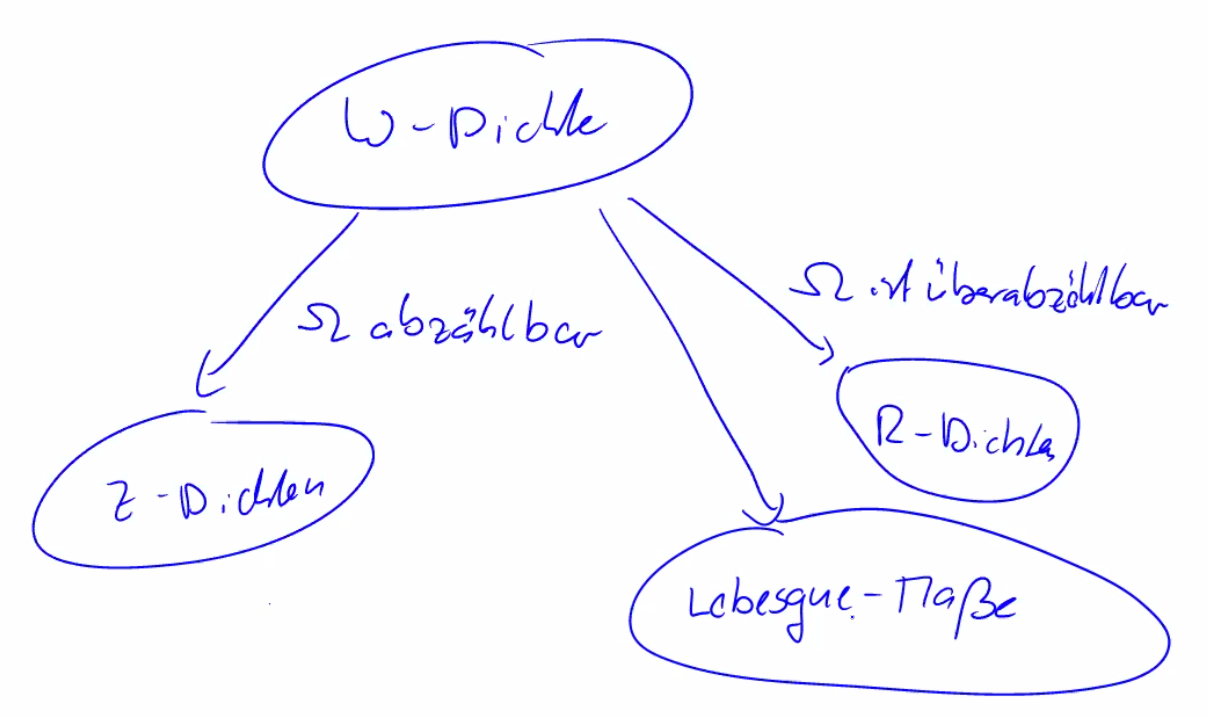
\includegraphics[width=256px]{diagram.png}\\
	Verteilungsfunktion:\\
	$\lim\limits_{x\to\infty} F(x)=1$\\
	$F\in C^0(\mathbb{R})$(Rechtsseitig stetig)\\
	gilt $0\leq F(x)\leq 1, Bild(f)\in[0,1]$\\
	$F$ ist monoton wachsend.\\
	Die wahrscheinlichkeitsdichtefunktion von $F$ ist $f(x)$:
	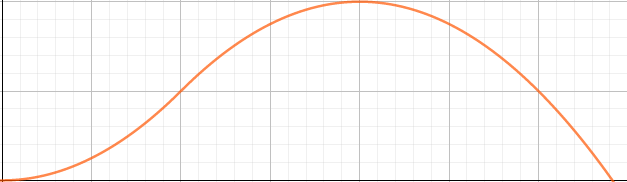
\includegraphics[width=256px]{funktionFvonf.png}\\
	\begin{itemize}
		\item Bernoulli
		\item Laplace
		\item geometrisch
		\item Poisson
		\item Normal
		\item Studentsche t-verteilung
		\item uniform
	\end{itemize}
	$q\in(0,1)$, $f(k)=(1-q)q^k\forall k\in\mathbb{N}$\\
	$P(\mathbb{N}) = P(\sum\limits_{k=1}^\infty \{k\}) = \sum\limits_{k=1}^\infty P(\{k\}) = \sum\limits_{k=1}^\infty f(k) = \sum\limits_{k=1}^\infty (1-q)q^k = (1-q)\sum\limits_{k=1}^\infty q^k = (1-q)\cdot \frac{1}{1-q}=1$. Also ist die Verteilung eine Zähldichte (weil $P(k)\geq 0,\forall k$ gilt, so auch jede partialsumme)\\
	Gemischte Verteilung:\\
	$P(x)=\alpha_D P_D(x)+\alpha_R P_R(x)$ mit $\alpha_D+\alpha_R = 1$\\
	(also eine linearkombination einer kontinuierlichen und diskreten verteilung)\\
	Verteilungsfunktion:\\
	$F(x):= P((-\infty,x]), x\in\mathbb{R}$ ist die Verteilungsfunktion von P.\\
	Es gilt $P((a,b])=F(b)-F(a)$\\
	$F(x)=\int\limits^x_{-\infty} f(t)dt\implies P((a,b])=F(b)-F(a)$\\
	Wenn F die VF eines W-Maßes P ist, dann gilt:\\
	\begin{itemize}
	\item F ist isoton (d.h. nicht monoton fallend)
	\item F ist normiert mit Grenzwerten $0$ und 1
	\item F ist rechtsseitig stetig
	\item F bisitzt linksseite Grenzwerte $F(x-)=\lim\limits_{h\to 0^+} F(x-h) = P((\infty,x))$
	\item Für die Einpunktmenge gilt $P(\{x\}) = F(x)-F(x-)$
	\end{itemize}
	\section{Normalverteilung}
	$f(x) = \frac{1}{\sigma\sqrt{2\pi}} e^{-\frac{(x-a)^2}{2\sigma^2}}$ $x\in\mathbb{R}$\\
	man schreibt $\mathscr{N}(\mu,\sigma^2)$ diese Verteilung ist additiv mit anderen Normalverteilungen\\
	$\mathscr{N}(\mu_1,\sigma^2_1)+\mathscr{N}(\mu_2,\sigma^2_1) = \mathscr{N}(\mu_2+\mu_1,\sigma^2_1+\sigma^2_2)$\\
	Die Verteilungsfunktion ist $\Phi(x) = \int ^x_\infty \frac{1}{\sqrt{2\pi}}e^{-\frac{u^2}{2}} du, x\in\mathbb{R
	}$\\
	also $\Phi(\frac{x-\mu}{\sigma})$ für eine $\mathscr{N}(\mu,\sigma)$\\
	$\Phi$ ist nur für positive Werte definiert, allerdings gilt $\Phi(-x)=1-\Phi(x)$\\
\end{document}